\setcounter{framenumber}{0}
%23

\begin{frame}
  \titlepage
\end{frame}

\begin{frame}{Learning Goals}
By the end of this lecture, students should be able to:
\begin{itemize}
    \item define the standard Normal distribution;
    \item standardize a Normal random variable;
    \item compute Normal probabilities using the standard Normal CDF;
    \item use the 68--95--99.7 rule;
    \item define the Exponential distribution;
    \item compute Exponential probabilities;
    \item understand the memoryless property of the Exponential distribution.
\end{itemize}
\end{frame}

\lecturepart{Normal Distribution}
\begin{frame}{The Normal Distribution $N(\mu,\sigma^2)$}

\begin{columns}[c]

\column{0.5\textwidth}

\begin{keybox}{Definition}
A continuous random variable \(X\) has a Normal distribution with mean \(\mu\) and variance \(\sigma^2\) if
\[
X\sim N(\mu,\sigma^2),
\]
and its density is
\[
f(x)
=
\frac{1}{\sqrt{2\pi\sigma^2}}
\exp\left(
-\frac{(x-\mu)^2}{2\sigma^2}
\right),
\qquad x\in\mathbb{R}.
\]
\end{keybox}

\column{0.5\textwidth}

\begin{center}
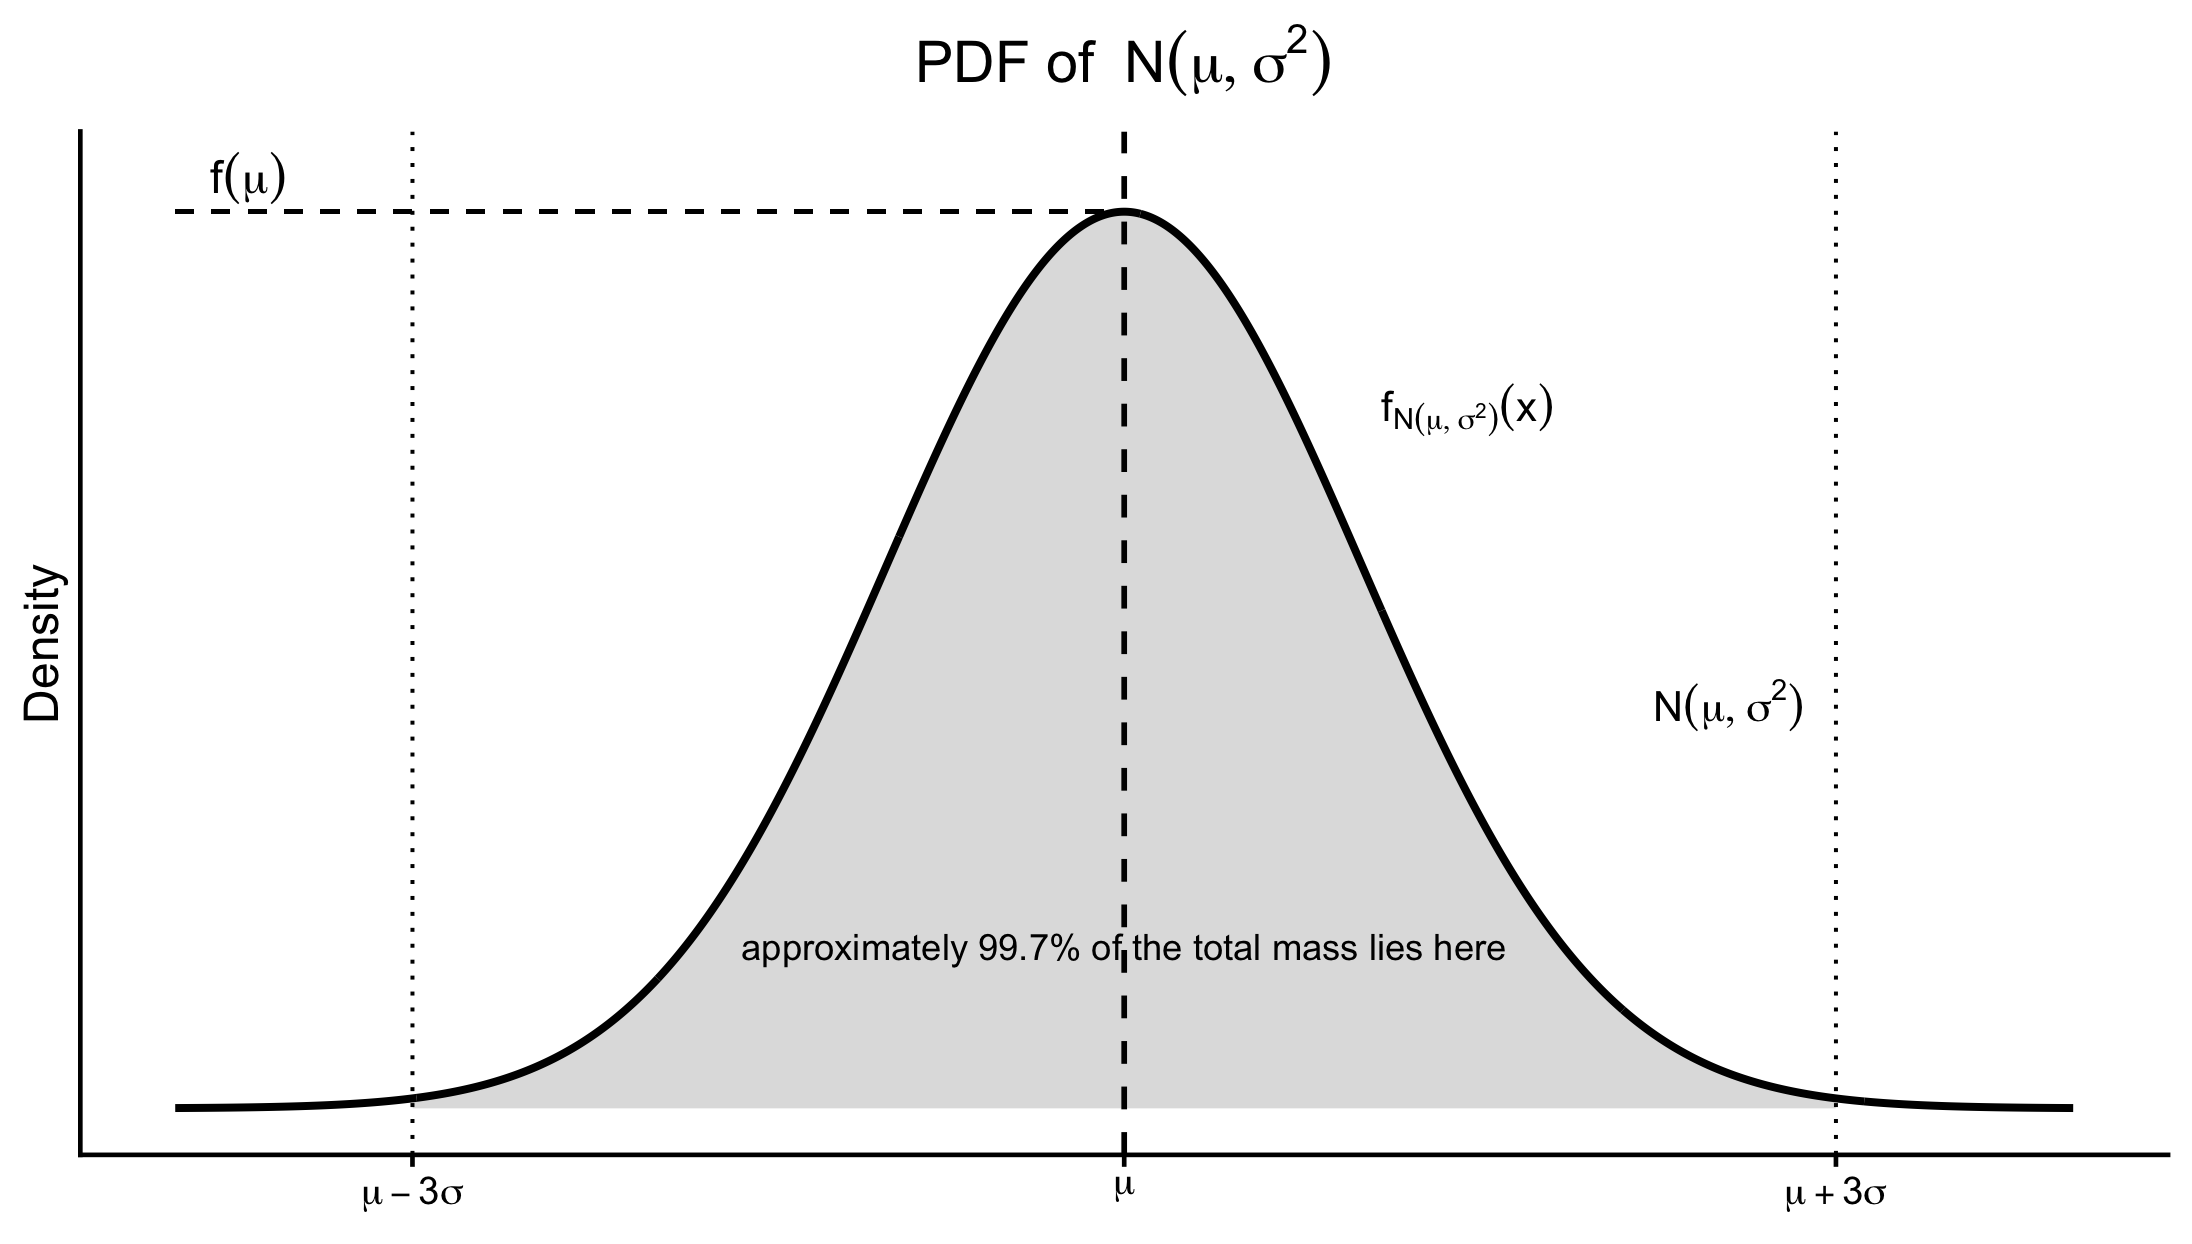
\includegraphics[width=\textwidth]{assets/figures/normalpdf.png}
\end{center}

\end{columns}

\vspace{0.2cm}

The parameter \(\mu\) controls the center, while \(\sigma^2\) controls the spread. The special case where $\mu=0$, $\sigma=1$ is called Standard Normal.

\begin{keybox}{Preview}
This is the most fundamental distribution in probability, with so many important fetures. Central Limit Theorem (CLT) will later shows one of its key aspects.
\end{keybox}

\end{frame}









\begin{frame}{PDF Verification of Normal}
\small
$f_X(x)\geq 0 $ is straightforward, so it suffices to show
\begin{keybox}{Claim} 
\[
\int_{-\infty}^{\infty} e^{-x^2/2}\,dx=\sqrt{2\pi}.
\]
\end{keybox}

Let
\[
I=\int_{-\infty}^{\infty}e^{-x^2/2}\,dx.
\]
Then
\[
I^2
=
\left(\int_{-\infty}^{\infty}e^{-x^2/2}\,dx\right)
\left(\int_{-\infty}^{\infty}e^{-y^2/2}\,dy\right)
=
\int_{\mathbb{R}^2}e^{-(x^2+y^2)/2}\,dx\,dy.
\]

Using polar coordinates,
\[
x=r\cos\theta,
\qquad
y=r\sin\theta,
\qquad
dx\,dy=r\,dr\,d\theta.
\]

Therefore,
\[
I^2
=
\int_0^{2\pi}\int_0^\infty e^{-r^2/2}r\,dr\,d\theta.
\]
Let \(u=r^2/2\), so \(du=r\,dr\). Then
\[
I^2
=
\int_0^{2\pi}\int_0^\infty e^{-u}\,du\,d\theta
=
\int_0^{2\pi}1\,d\theta
=
2\pi.
\]
Thus,
\[
{I=\sqrt{2\pi}}.
\]

\end{frame}






















\begin{frame}{Mean and Variance of \(N(\mu,\sigma^2)\)}

\begin{keybox}{Proposition}


Suppose
\[
X\sim N(\mu,\sigma^2),
\]
with density
\[
f(x)
=
\frac{1}{\sqrt{2\pi\sigma^2}}
\exp\left(
-\frac{(x-\mu)^2}{2\sigma^2}
\right).
\]

Then,

\[
\mathbb{E}(X)=\mu,
\qquad
\operatorname{Var}(X)=\sigma^2.
\]
\end{keybox}

\vspace{0.25cm}

Proof: By definition,
\[
\mathbb{E}(X)
=
\int_{-\infty}^{\infty}
x f(x)\,dx.
\]
\end{frame}


\begin{frame}{}
Let
\[
z=x-\mu.
\]
Then
\[
x=z+\mu,
\qquad
dx=dz.
\]

Therefore,
\[
\mathbb{E}(X)
=
\int_{-\infty}^{\infty}
(z+\mu)
\frac{1}{\sqrt{2\pi\sigma^2}}
e^{-z^2/(2\sigma^2)}
\,dz.
\]

Splitting the integral,
\[
\mathbb{E}(X)
=
\underbrace{
\int_{-\infty}^{\infty}
z
\frac{1}{\sqrt{2\pi\sigma^2}}
e^{-z^2/(2\sigma^2)}
\,dz
}_{=0}
+
\mu
\underbrace{
\int_{-\infty}^{\infty}
\frac{1}{\sqrt{2\pi\sigma^2}}
e^{-z^2/(2\sigma^2)}
\,dz
}_{=1}.
\]

Hence,
\[
{\mathbb{E}(X)=\mu.}
\]

\end{frame}







\begin{frame}{Variance of \(N(\mu,\sigma^2)\)}

Recall:
\[
\operatorname{Var}(X)
=
\mathbb{E}\big[(X-\mu)^2\big].
\]

Using LOTUS,
\[
\operatorname{Var}(X)
=
\int_{-\infty}^{\infty}
(x-\mu)^2
f(x)\,dx.
\]

Let
\[
z=x-\mu.
\]

Then
\[
\operatorname{Var}(X)
=
\int_{-\infty}^{\infty}
z^2
\frac{1}{\sqrt{2\pi\sigma^2}}
e^{-z^2/(2\sigma^2)}
\,dz.
\]

Now substitute
\[
u=\frac{z}{\sigma},
\qquad
z=\sigma u,
\qquad
dz=\sigma\,du.
\]

Then
\[
\operatorname{Var}(X)
=
\sigma^2
\int_{-\infty}^{\infty}
u^2
\frac{1}{\sqrt{2\pi}}
e^{-u^2/2}
\,du.
\]

The remaining integral equals \(1\), since it is the variance of the standard Normal distribution \(N(0,1)\).

Therefore,
\[
{
\operatorname{Var}(X)=\sigma^2.
}
\]

\end{frame}
















\begin{frame}{Standard Normal CDF}
The standard Normal CDF is denoted by
\[
\Phi(z).
\]

It is defined by
\[
\Phi(z)
=
\Prob(Z\leq z)
=
\int_{-\infty}^{z}
\frac{1}{\sqrt{2\pi}}e^{-t^2/2}\,dt.
\]

\vspace{0.25cm}

\begin{keybox}{Important}
There is no elementary closed-form expression for $\Phi(z)$.
\end{keybox}

So Normal probabilities are usually computed using tables, calculators, or software. See "normal-table.pdf" in Canvas for the Standard Normal table.
\end{frame}

\begin{frame}{Symmetry of the Standard Normal}
The standard Normal PDF is symmetric about $0$, i.e.,  $\varphi(z)=\varphi(-z)$. Therefore, $\Prob(Z\leq -z)=\Prob(Z\geq z)$. In terms of the CDF, $\Phi(-z)=1-\Phi(z).
$ This is why some Normal CDF tables skip the negative values and only provide $\phi(z)$ for $z\geq 0$.



\begin{center}
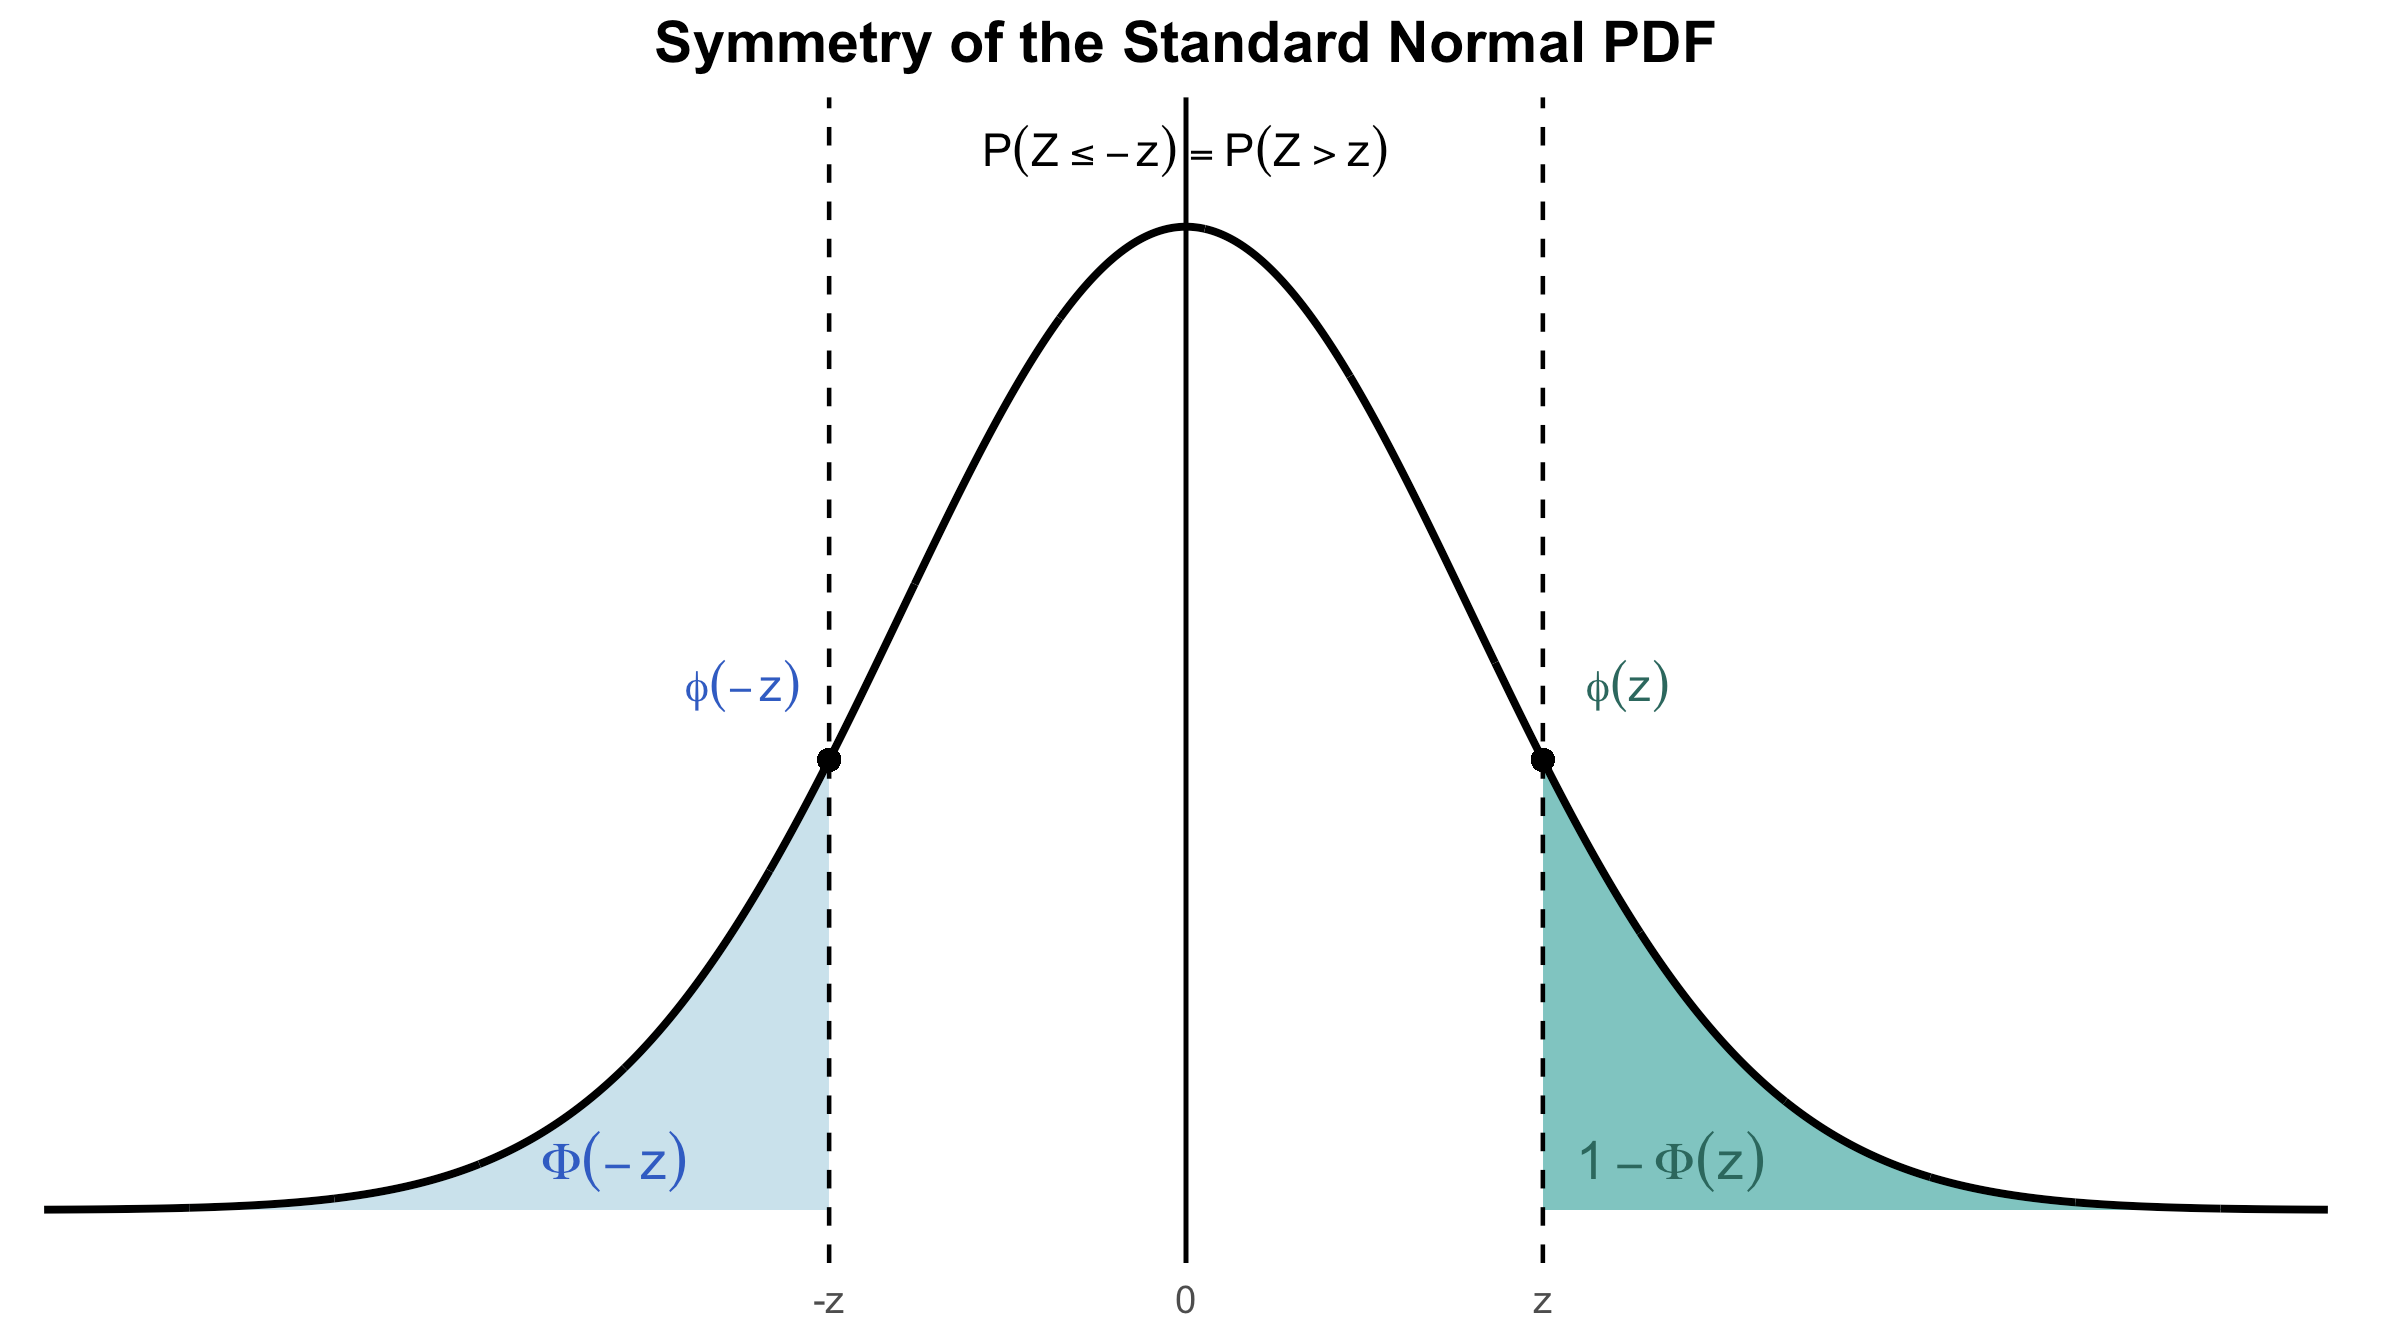
\includegraphics[width=0.6\textwidth]{assets/figures/tails.png}
\end{center}



\end{frame}

\begin{frame}{Converting $N(0,1)$  to $N(\mu,\sigma^2)$ }
\begin{keybox}{Proposition}
If
\[
Z\sim N(0,1),
\]
then
\[
X=\mu+\sigma Z
\]
has the Normal distribution with mean $\mu$ and variance $\sigma^2$, i.e.,

\[
X\sim N(\mu,\sigma^2).
\]
\end{keybox}
\end{frame}

\begin{frame}{Converting $N(\mu,\sigma^2)$  to  $N(0,1)$  }


\begin{keybox}{Proposition}

If
\[
X\sim N(\mu,\sigma^2),
\]
then
\[
\boxed{
Z=\frac{X-\mu}{\sigma}\sim N(0,1).
}
\]
\end{keybox}
\vspace{0.25cm}

Standardization converts a general Normal random variable into a standard Normal.

\vspace{0.25cm}

\begin{keybox}{Use}
To compute probabilities involving $X$, convert them into probabilities involving $Z$, and then use the Normal probability table.
\end{keybox}
\end{frame}

\begin{frame}{Example: Standardizing}
Suppose
\[
X\sim N(70,10^2).
\]

Find
\[
\Prob(X<85).
\]

Standardize:
\[
\Prob(X<85)
=
\Prob\left(
\frac{X-70}{10}<\frac{85-70}{10}
\right).
\]

Thus
\[
\Prob(X<85)=\Prob(Z<1.5)=\Phi(1.5).
\]
\end{frame}

\begin{frame}{The 68--95--99.7 Rule}
If
\[
X\sim N(\mu,\sigma^2),
\]
then approximately:

\[
\Prob(|X-\mu|<\sigma)\approx 0.68,
\]

\[
\Prob(|X-\mu|<2\sigma)\approx 0.95,
\]

\[
\Prob(|X-\mu|<3\sigma)\approx 0.997.
\]

\vspace{0.25cm}

\begin{keybox}{Interpretation}
Most Normal observations lie within a few standard deviations of the mean.
\end{keybox}
\end{frame}









%%%%%%%%%%%%%%%%%%%%%%%%%%%%%%%%%%%%%%%%%%%%%%%%%%%%%%%%%%%%%%%%%%%%%%%%%%%%%%%
% NORMAL APPROXIMATION TO THE BINOMIAL
%%%%%%%%%%%%%%%%%%%%%%%%%%%%%%%%%%%%%%%%%%%%%%%%%%%%%%%%%%%%%%%%%%%%%%%%%%%%%%%

\lecturepart{Normal Approximation to the Binomial}


% ---------------------------------------------------------------------------
\begin{frame}{Motivation: Large Binomial Probabilities}

Suppose
\[
X\sim\operatorname{Bin}(n,p).
\]

For a single value \(k\), we can compute
\[
\Prob(X=k)
=
\binom{n}{k}p^k(1-p)^{n-k}.
\]

However, probabilities such as
\[
\Prob(X\leq k)
=
\sum_{j=0}^{k}
\binom{n}{j}p^j(1-p)^{n-j}
\]
may require adding a very large number of terms.

\vspace{0.25cm}

\begin{keybox}{Main idea}
When \(n\) is sufficiently large, the Binomial distribution is approximately
Normal.
\end{keybox}

Thus, complicated Binomial sums can often be approximated using the standard
Normal CDF \(\Phi\).

\end{frame}


% ---------------------------------------------------------------------------
\begin{frame}{Why Does the Normal Approximation Work?}

A Binomial random variable can be written as
\[
X=X_1+\cdots+X_n,
\]
where
\[
X_i=
\begin{cases}
1, & \text{if trial \(i\) is a success},\\
0, & \text{if trial \(i\) is a failure}.
\end{cases}
\]

The variables \(X_1,\ldots,X_n\) are independent Bernoulli random variables
with
\[
\mathbb{E}(X_i)=p,
\qquad
\operatorname{Var}(X_i)=p(1-p).
\]

Therefore,
\[
\mathbb{E}(X)=np,
\qquad
\operatorname{Var}(X)=np(1-p).
\]

\vspace{0.2cm}

As \(n\) becomes large, the distribution of the sum
\[
X_1+\cdots+X_n
\]
becomes approximately bell-shaped.

\begin{keybox}{Preview}
This is a consequence of the Central Limit Theorem, which will be studied
later.
\end{keybox}

\end{frame}


% ---------------------------------------------------------------------------
\begin{frame}{Normal Approximation to the Binomial}

\begin{keybox}{Approximation}
Suppose
\[
X\sim\operatorname{Bin}(n,p).
\]

When \(n\) is sufficiently large and \(p\) is not too close to \(0\) or \(1\),
we may use the approximation
\[
\boxed{
X\approx Y,
\qquad
Y\sim N\bigl(np,np(1-p)\bigr).
}
\]
\end{keybox}

Thus, the approximating Normal random variable has the same mean and variance
as the Binomial random variable:
\[
\mu=np,
\qquad
\sigma^2=np(1-p),
\qquad
\sigma=\sqrt{np(1-p)}.
\]

\vspace{0.25cm}

After applying a continuity correction, we standardize using
\[
Z=\frac{Y-np}{\sqrt{np(1-p)}}.
\]

\end{frame}


\begin{frame}{Normal Approximation to the Binomial}
\begin{center}
    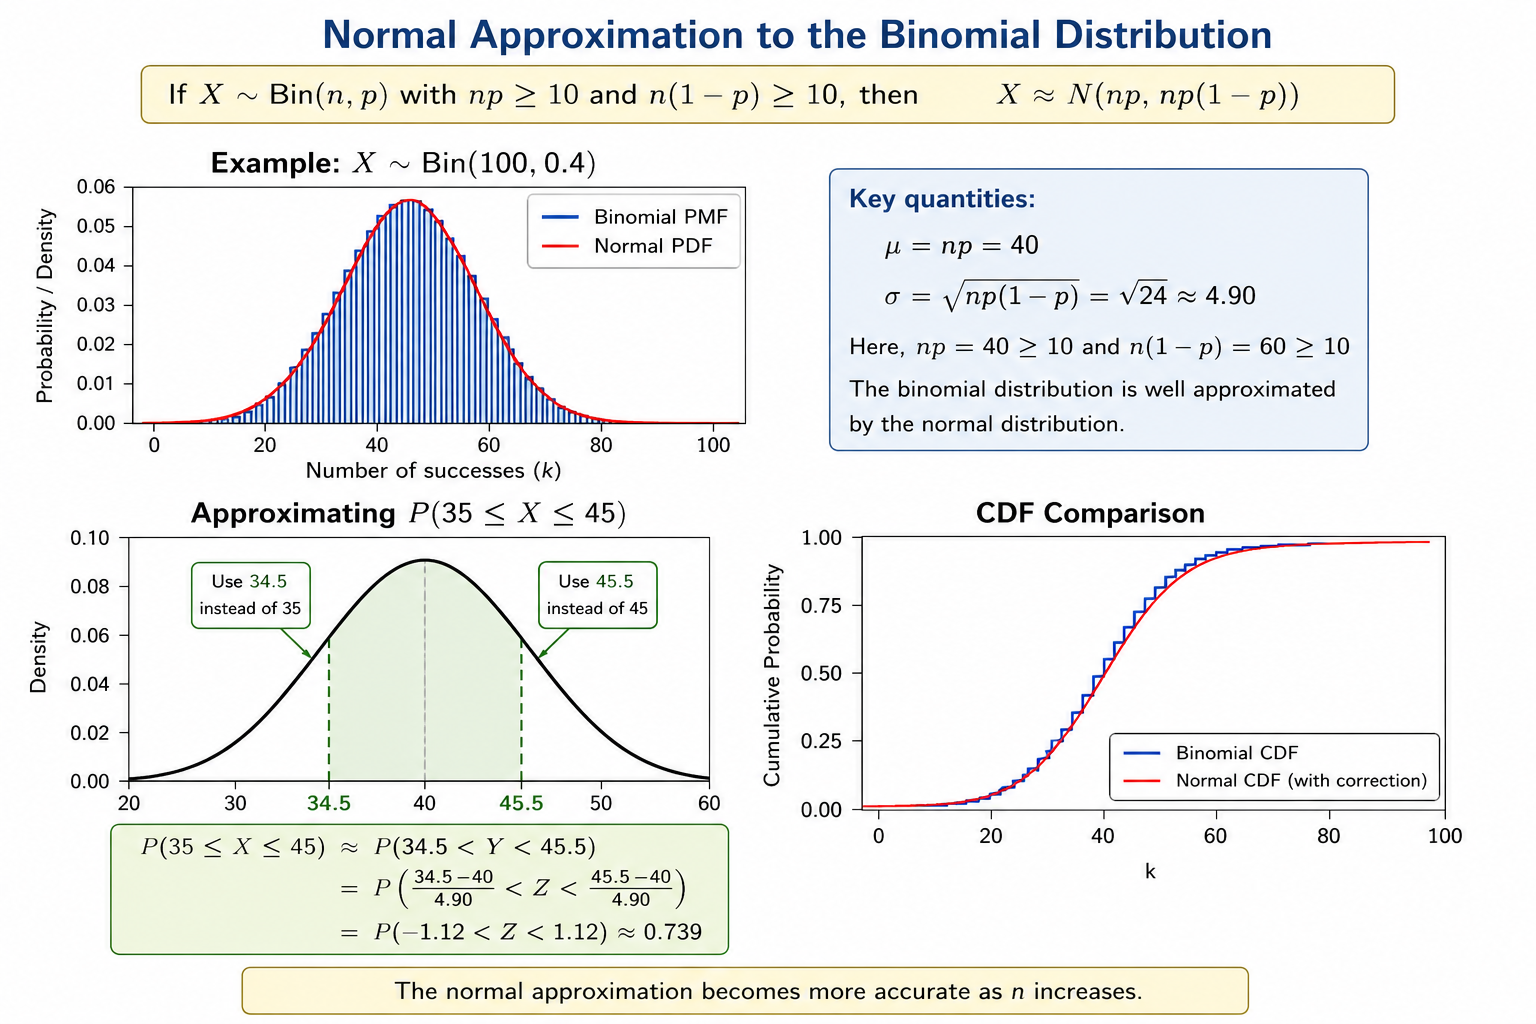
\includegraphics[
        width=\textwidth,
        height=0.9\textheight,
        keepaspectratio
    ]{assets/figures/normal-binomial-approximation.png}
\end{center}
\end{frame}


% ---------------------------------------------------------------------------
\begin{frame}{When Is the Approximation Appropriate?}

A commonly used rule is to require
\[
\boxed{
np\geq 10
\qquad\text{and}\qquad
n(1-p)\geq 10.
}
\]

These quantities represent the expected numbers of successes and failures.

\vspace{0.3cm}

\begin{keybox}{Interpretation}
The approximation works best when we expect sufficiently many successes and
sufficiently many failures.
\end{keybox}

\vspace{0.25cm}

If \(p\) is very close to \(0\), the Binomial distribution is strongly
right-skewed.

If \(p\) is very close to \(1\), the Binomial distribution is strongly
left-skewed.

In either case, a symmetric Normal curve may provide a poor approximation.

\end{frame}


% ---------------------------------------------------------------------------
\begin{frame}{Why Is a Continuity Correction Needed?}

A Binomial random variable is discrete:
\[
X\in\{0,1,2,\ldots,n\}.
\]

A Normal random variable is continuous:
\[
Y\in\mathbb{R}.
\]

For example, the event \(X=5\) is represented by the interval centered at
\(5\):
\[
4.5<Y<5.5.
\]

Thus,
\[
\Prob(X=5)
\approx
\Prob(4.5<Y<5.5).
\]

\vspace{0.25cm}

\begin{keybox}{Continuity correction}
To translate a discrete boundary into a continuous boundary, shift the
endpoint by \(0.5\).
\end{keybox}

\end{frame}


% ---------------------------------------------------------------------------
\begin{frame}{Continuity-Correction Rules}

Let
\[
X\sim\operatorname{Bin}(n,p),
\qquad
Y\sim N\bigl(np,np(1-p)\bigr).
\]

Once standardized, the following approximations are used:

\[
\begin{array}{c|c}
\text{Binomial probability}
&
\text{Normal approximation}
\\[0.1cm]
\hline
\Prob(X=k)
&
\Prob(k-0.5<Y<k+0.5)
\\[0.15cm]
\Prob(X\leq k)
&
\Prob(Y<k+0.5)
\\[0.15cm]
\Prob(X<k)
&
\Prob(Y<k-0.5)
\\[0.15cm]
\Prob(X\geq k)
&
\Prob(Y>k-0.5)
\\[0.15cm]
\Prob(X>k)
&
\Prob(Y>k+0.5)
\\[0.15cm]
\Prob(a\leq X\leq b)
&
\Prob(a-0.5<Y<b+0.5)
\end{array}
\]

\end{frame}



% ---------------------------------------------------------------------------
\begin{frame}{Procedure for the Normal Approximation}

Suppose
\[
X\sim\operatorname{Bin}(n,p).
\]

\begin{enumerate}
    \item Check if the conditions hold
    \[
    np\geq 10,
    \qquad
    n(1-p)\geq 10.
    \]

    \item Compute
    \[
    \mu=np,
    \qquad
    \sigma=\sqrt{np(1-p)}.
    \]

    \item Apply the continuity correction.

    \item Standardize using
    \[
    Z=\frac{Y-\mu}{\sigma}.
    \]

    \item Use the standard Normal CDF \(\Phi\).
\end{enumerate}

\begin{keybox}{Important}
The continuity correction must be applied before standardizing.
\end{keybox}

\end{frame}


% ---------------------------------------------------------------------------
\begin{frame}{Example: A Binomial Probability}

Suppose
\[
X\sim\operatorname{Bin}(100,0.4).
\]

Approximate
\[
\Prob(35\leq X\leq 45).
\]

First,
\[
np=40,
\qquad
n(1-p)=60,
\]
so the Normal approximation is appropriate.

The mean and standard deviation are
\[
\mu=100(0.4)=40,
\]
and
\[
\sigma
=
\sqrt{100(0.4)(0.6)}
=
\sqrt{24}.
\]

Using the continuity correction,
\[
\Prob(35\leq X\leq45)
\approx
\Prob(34.5<Y<45.5),
\]
where
\[
Y\sim N(40,24).
\]

\end{frame}


% ---------------------------------------------------------------------------
\begin{frame}{Example: A Binomial Probability, Continued}

Standardizing gives
\[
\Prob(34.5<Y<45.5)
=
\Prob\left(
\frac{34.5-40}{\sqrt{24}}
<
Z
<
\frac{45.5-40}{\sqrt{24}}
\right).
\]

Therefore,
\[
\Prob(35\leq X\leq45)
\approx
\Prob(-1.123<Z<1.123).
\]

Using the standard Normal CDF,
\[
\Prob(-1.123<Z<1.123)
=
\Phi(1.123)-\Phi(-1.123).
\]

By symmetry,
\[
\Phi(-1.123)=1-\Phi(1.123).
\]

Thus,
\[
\Prob(35\leq X\leq45)
\approx
2\Phi(1.123)-1
\approx
0.739.
\]

\end{frame}


%%%%%%%%%%%%%%%%%%%%%%%%%%%%%%%%%%%%%%%%%%%%%%%%%%%%%%%%%%%%%%%%%%%%%%%%%%%%%%%
% EXAMPLES FROM GHAHRAMANI
%%%%%%%%%%%%%%%%%%%%%%%%%%%%%%%%%%%%%%%%%%%%%%%%%%%%%%%%%%%%%%%%%%%%%%%%%%%%%%%


% ---------------------------------------------------------------------------
\begin{frame}{Example: Stocking a Bestseller}

Suppose that the odds are 1 to 5000 in favor of a customer buying a particular fiction bestseller.

If \(800\) customers enter the store every day, how many copies should the
store stock each month so that, with probability greater than \(98\%\), it
does not run out?

Assume that a month has \(30\) days.

\vfill

{\scriptsize
Source: Saeed Ghahramani, \emph{Fundamentals of Probability}.
}

\end{frame}


% ---------------------------------------------------------------------------
\begin{frame}{Solution: Stocking a Bestseller}

Let
\[
X=\text{number of customers who buy the book during the month}.
\]

The total number of customers is
\[
n=30(800)=24000.
\]
 

Therefore,
\[
X\sim\operatorname{Bin}\left(24000,\frac{1}{5000 + 1}\right).
\]

The expected number of buyers is
\[
np
=
\frac{24000}{5000}
\approx
4.799.
\]

However,
\[
np<10.
\]

\begin{keybox}{Conclusion}
The usual Normal approximation is not appropriate because the expected
number of successes is too small.
\end{keybox}

\end{frame}


% ---------------------------------------------------------------------------
\begin{frame}{Solution: Using a Poisson Approximation}

Since \(n\) is large and \(p\) is very small, the Binomial distribution is
better approximated by a Poisson distribution:
\[
X\approx\operatorname{Pois}(\lambda),
\qquad
\lambda=np\approx4.799.
\]

If the bookstore stocks \(m\) copies, it does not run out when
\[
X\leq m.
\]

We seek the smallest integer \(m\) such that
\[
\Prob(X\leq m)>0.98.
\]

Using the Poisson CDF,
\[
\Prob(X\leq9)
\approx
\sum_{k=0}^{9}
e^{-4.799}\frac{4.799^k}{k!}
\approx
0.975,
\]
which is less than \(0.98\).

However,
\[
\Prob(X\leq10)
\approx
\sum_{k=0}^{10}
e^{-4.799}\frac{4.u8^k}{k!}
\approx
0.990.
\]

Therefore, the store should stock
\[
\boxed{10\text{ copies}.}
\]

\end{frame}

% ---------------------------------------------------------------------------
\begin{frame}{Example: Sampling Light Bulbs}

Every day, a factory produces \(5000\) light bulbs, of which \(2500\) are
Type I and \(2500\) are Type II.

A sample of \(40\) light bulbs is selected at random without replacement.

What is the approximate probability that the sample contains at least
\(18\) light bulbs of each type?

\vfill

{\scriptsize
Source: Saeed Ghahramani, \emph{Fundamentals of Probability}.
}

\end{frame}


% ---------------------------------------------------------------------------
\begin{frame}{Solution: Defining the Random Variable}

Let
\[
X=\text{number of Type I bulbs in the sample}.
\]

Exactly,
\[
X\sim\operatorname{Hypergeo}(5000,2500,40).
\]

Because the sample size is small relative to the population size,
\[
\frac{40}{5000}=0.008,
\]
sampling without replacement is approximately equivalent to sampling with
replacement.

Thus,
\[
X
\approx
\operatorname{Bin}\left(40,\frac{2500}{5000}\right)
=
\operatorname{Bin}\left(40,\frac12\right).
\]

We have
\[
np=20,
\qquad
n(1-p)=20,
\]
so the Normal approximation is appropriate.

\end{frame}


% ---------------------------------------------------------------------------
\begin{frame}{Solution: Translating the Event}

If the sample contains \(X\) Type I bulbs, then it contains
\[
40-X
\]
Type II bulbs.

We require at least \(18\) bulbs of each type:
\[
X\geq18
\]
and
\[
40-X\geq18.
\]

The second inequality gives
\[
X\leq22.
\]

Therefore, the desired event is
\[
18\leq X\leq22.
\]

For the Binomial approximation,
\[
\mu=np=20,
\]
and
\[
\sigma^2=np(1-p)=10.
\]

Thus,
\[
X\approx Y,
\qquad
Y\sim N(20,10).
\]

\end{frame}


% ---------------------------------------------------------------------------
\begin{frame}{Solution: Applying the Continuity Correction}

Using the continuity correction,
\[
\Prob(18\leq X\leq22)
\approx
\Prob(17.5<Y<22.5).
\]

Standardizing,
\[
\Prob(17.5<Y<22.5)
=
\Prob\left(
\frac{17.5-20}{\sqrt{10}}
<
Z
<
\frac{22.5-20}{\sqrt{10}}
\right).
\]

Since
\[
\frac{2.5}{\sqrt{10}}
\approx0.791,
\]
we obtain
\[
\Prob(18\leq X\leq22)
\approx
\Prob(-0.791<Z<0.791).
\]

Therefore,
\[
\Prob(18\leq X\leq22)
\approx
\Phi(0.791)-\Phi(-0.791).
\]

\end{frame}


% ---------------------------------------------------------------------------
\begin{frame}{Solution: Final Probability}

Using symmetry,
\[
\Phi(-0.791)=1-\Phi(0.791).
\]

Hence,
\[
\Prob(-0.791<Z<0.791)
=
2\Phi(0.791)-1.
\]

Using
\[
\Phi(0.791)\approx0.785,
\]
we obtain
\[
2(0.785)-1
\approx
0.570.
\]

Therefore,
\[
\boxed{
\Prob(\text{at least 18 bulbs of each type})
\approx0.570.
}
\]

\begin{keybox}{Interpretation}
There is approximately a \(57\%\) probability that the sample contains
between \(18\) and \(22\) Type I bulbs, and hence at least \(18\) bulbs of
each type.
\end{keybox}

\end{frame}


%%%%%%%%%%%%%%%%%%%%%%%%%%%%%%%%%%%%%%%%%%%%%%%%%%%%%%%%%%%%%%%%%%%%%%%%%%%%%%%
% DIRECT NORMAL-DISTRIBUTION EXAMPLES
%%%%%%%%%%%%%%%%%%%%%%%%%%%%%%%%%%%%%%%%%%%%%%%%%%%%%%%%%%%%%%%%%%%%%%%%%%%%%%%


% ---------------------------------------------------------------------------
\begin{frame}{Example: A Company's Lifetime Claim}

Suppose that the lifetimes of light bulbs produced by a company are Normal
random variables with mean \(1000\) hours and standard deviation \(100\)
hours.

The company claims that \(95\%\) of its light bulbs last at least \(900\)
hours.

Is the company's claim correct?

\vfill

{\scriptsize
Source: Saeed Ghahramani, \emph{Fundamentals of Probability}.
}

\end{frame}


% ---------------------------------------------------------------------------
\begin{frame}{Solution: A Company's Lifetime Claim}

Let
\[
X=\text{lifetime of a randomly selected light bulb}.
\]

Then
\[
X\sim N(1000,100^2).
\]

We compute
\[
\Prob(X\geq900).
\]

Standardizing,
\[
\Prob(X\geq900)
=
\Prob\left(
Z\geq
\frac{900-1000}{100}
\right).
\]

Therefore,
\[
\Prob(X\geq900)
=
\Prob(Z\geq-1).
\]

By symmetry,
\[
\Prob(Z\geq-1)=\Phi(1).
\]

Thus,
\[
\Prob(X\geq900)
\approx0.8413.
\]

\end{frame}


% ---------------------------------------------------------------------------
\begin{frame}{Solution: Evaluating the Claim}

The actual probability is
\[
\Prob(X\geq900)\approx0.8413.
\]

Thus, approximately \(84.13\%\) of the bulbs last at least \(900\) hours.

The company claims that the percentage is \(95\%\).

Since
\[
0.8413<0.95,
\]
the claim is incorrect.

\[
\boxed{\text{No, the company's claim is not correct.}}
\]

\begin{keybox}{Remark}
A lifetime of \(900\) hours is only one standard deviation below the mean.
For a Normal distribution, approximately \(84\%\), not \(95\%\), of the
observations lie above this point.
\end{keybox}

\end{frame}


% ---------------------------------------------------------------------------
\begin{frame}{Example: Bulbs from Two Companies}

The lifetime of a bulb produced by the first company is Normal with mean
\(1000\) hours and standard deviation \(100\) hours.

The lifetime of a bulb produced by the second company is Normal with mean
\(900\) hours and standard deviation \(150\) hours.

Howard buys one bulb from each company.

Assuming the two lifetimes are independent, what is the probability that at
least one bulb lasts \(980\) or more hours?

\vfill

{\scriptsize
Source: Saeed Ghahramani, \emph{Fundamentals of Probability}.
}

\end{frame}


% ---------------------------------------------------------------------------
\begin{frame}{Solution: Defining the Lifetimes}

Let
\[
X=\text{lifetime of the bulb from the first company},
\]
and
\[
Y=\text{lifetime of the bulb from the second company}.
\]

Then
\[
X\sim N(1000,100^2),
\]
and
\[
Y\sim N(900,150^2).
\]

We want
\[
\Prob(X\geq980\ \text{or}\ Y\geq980).
\]

It is easier to use the complementary event:
\[
\Prob(X\geq980\ \text{or}\ Y\geq980)
=
1-\Prob(X<980,\ Y<980).
\]

Because \(X\) and \(Y\) are independent,
\[
\Prob(X<980,\ Y<980)
=
\Prob(X<980)\Prob(Y<980).
\]

\end{frame}


% ---------------------------------------------------------------------------
\begin{frame}{Solution: First Company's Bulb}

For the first bulb,
\[
\Prob(X<980)
=
\Prob\left(
Z<
\frac{980-1000}{100}
\right).
\]

Thus,
\[
\Prob(X<980)
=
\Prob(Z<-0.2)
=
\Phi(-0.2).
\]

Using the Normal table,
\[
\Phi(-0.2)\approx0.4207.
\]

Therefore,
\[
\Prob(X<980)\approx0.4207.
\]

Equivalently,
\[
\Prob(X\geq980)
\approx
1-0.4207
=
0.5793.
\]

\end{frame}


% ---------------------------------------------------------------------------
\begin{frame}{Solution: Second Company's Bulb}

For the second bulb,
\[
\Prob(Y<980)
=
\Prob\left(
Z<
\frac{980-900}{150}
\right).
\]

Now,
\[
\frac{980-900}{150}
=
\frac{80}{150}
\approx0.533.
\]

Therefore,
\[
\Prob(Y<980)
=
\Phi(0.533)
\approx0.7031.
\]

Equivalently,
\[
\Prob(Y\geq980)
\approx
1-0.7031
=
0.2969.
\]

\end{frame}


% ---------------------------------------------------------------------------
\begin{frame}{Solution: At Least One Bulb}

Using independence,
\[
\Prob(X<980,\ Y<980)
=
\Prob(X<980)\Prob(Y<980).
\]

Thus,
\[
\Prob(X<980,\ Y<980)
\approx
(0.4207)(0.7031)
\approx
0.2958.
\]

Therefore,
\[
\Prob(X\geq980\ \text{or}\ Y\geq980)
\approx
1-0.2958.
\]

Hence,
\[
\boxed{
\Prob(\text{at least one lasts at least \(980\) hours})
\approx0.7042.
}
\]

\end{frame}


% ---------------------------------------------------------------------------
\begin{frame}{Normal Approximation: Summary}

Suppose
\[
X\sim\operatorname{Bin}(n,p).
\]

When
\[
np\geq10
\qquad\text{and}\qquad
n(1-p)\geq10,
\]
we use
\[
X\approx N\bigl(np,np(1-p)\bigr).
\]

The procedure is:

\begin{enumerate}
    \item Compute
    \[
    \mu=np,
    \qquad
    \sigma=\sqrt{np(1-p)}.
    \]

    \item Apply the continuity correction.

    \item Standardize:
    \[
    Z=\frac{Y-\mu}{\sigma}.
    \]

    \item Use \(\Phi\) to calculate the probability.
\end{enumerate}

\begin{keybox}{Important}
If \(np\) or \(n(1-p)\) is too small, another approximation, such as the
Poisson approximation, may be more appropriate.
\end{keybox}

\end{frame}







\lecturepart{Exponential Distribution}

\href{https://drive.google.com/file/d/1Qev6nT1mknMwBNL8iIOvS4Ev9mG2eKhW/view?usp=sharing}{Summary so far.}


\begin{frame}{Exponential Distribution}
The Exponential distribution models waiting times.

\vspace{0.25cm}

Examples:
\begin{itemize}
    \item waiting time until a phone call;
    \item waiting time until a radioactive particle decays;
    \item waiting time until a customer arrives;
    \item lifetime of certain components.
\end{itemize}

\vspace{0.25cm}

It is the continuous analog of waiting for the first success.
\end{frame}

\begin{frame}{Definition of Exponential Distribution}
\begin{keybox}{Definition}
A random variable $X$ has the Exponential distribution with rate $\lambda>0$ if its PDF is
\[
f(x)=
\lambda e^{-\lambda x},
\qquad x>0.
\]

We write
\[
X\sim \operatorname{Exp}(\lambda).
\]
\end{keybox}

For $x\leq0$,
\[
f(x)=0.
\]
\end{frame}

\begin{frame}{Exponential CDF and Survival Function}
If
\[
X\sim \operatorname{exp}(\lambda),
\]
then for $x>0$,

\[
F(x)=\Prob(X\leq x)=1-e^{-\lambda x}.
\]

Therefore,

\[
\Prob(X>x)=1-F(x)=e^{-\lambda x}.
\]

\vspace{0.25cm}

\begin{keybox}{Survival function}
\[
\boxed{
\Prob(X>x)=e^{-\lambda x}.
}
\]
\end{keybox}
\end{frame}











\begin{frame}{Mean and Variance of Exponential}
If
\[
X\sim \operatorname{Exp}(\lambda),
\]
then
\[
\mathbb{E}(X)=\frac{1}{\lambda},
\]
and
\[
\operatorname{Var}(X)=\frac{1}{\lambda^2}.
\]

\vspace{0.25cm}

\begin{keybox}{Interpretation}
A larger rate $\lambda$ means events occur more frequently, so waiting times become shorter on average.
\end{keybox}
\end{frame}



\begin{frame}{Proof of the Mean}
The density of an exponential random variable is
\[
f(x)=\lambda e^{-\lambda x},
\qquad x\ge0.
\]

Thus
\[
\mathbb{E}(X)
=
\int_0^\infty x\lambda e^{-\lambda x}\,dx.
\]

Use integration by parts.

Let
\[
u=x,
\qquad
dv=\lambda e^{-\lambda x}\,dx.
\]

Then
\[
du=dx,
\qquad
v=-e^{-\lambda x}.
\]

Therefore,
\[
\mathbb{E}(X)
=
\left[
-x e^{-\lambda x}
\right]_0^\infty
+
\int_0^\infty e^{-\lambda x}\,dx.
\]

The boundary term equals $0$, so
\[
\mathbb{E}(X)
=
\int_0^\infty e^{-\lambda x}\,dx
=
\left[
-\frac1\lambda e^{-\lambda x}
\right]_0^\infty.
\]

Hence
\[
\mathbb{E}(X)=\frac1\lambda.
\]
\end{frame}



\begin{frame}{Proof of the Variance}
We first compute
\[
\mathbb{E}(X^2).
\]

Using the density,
\[
\mathbb{E}(X^2)
=
\int_0^\infty x^2\lambda e^{-\lambda x}\,dx.
\]

Applying integration by parts twice gives
\[
\mathbb{E}(X^2)=\frac{2}{\lambda^2}.
\]

Now use
\[
\operatorname{Var}(X)
=
\mathbb{E}(X^2)-(\mathbb{E}(X))^2.
\]

Therefore,
\[
\operatorname{Var}(X)
=
\frac{2}{\lambda^2}
-
\left(\frac1\lambda\right)^2.
\]

Hence
\[
\operatorname{Var}(X)
=
\frac1{\lambda^2}.
\]
\end{frame}

\begin{frame}{Memoryless Property of $Exp(\lambda)$}
\begin{keybox}{Memoryless Property}
If
\[
X\sim \operatorname{exp}(\lambda),
\]
then for $s,t\geq0$,

\[
{
\Prob(X>s+t\mid X>s)=\Prob(X>t).
}
\]
\end{keybox}

\vspace{0.25cm}

Interpretation:

Given that we have already waited $s$ units of time, the additional waiting time behaves like a fresh Exponential random variable. In other words, how long you have already waited does not affect how much longer you will need to wait

\textbf{Remark}: Exponential distribution is the only memoryless r.v. among all the continuous r.v.s. Also, the only memoryless discrete r.v. is the Geometric r.v. that we studied in Chapter 3. 
\end{frame}

\begin{frame}{Proof of Memorylessness}
Using conditional probability,

\[
\Prob(X>s+t\mid X>s)
=
\frac{\Prob(X>s+t)}{\Prob(X>s)}.
\]

For an Exponential random variable,

\[
\Prob(X>x)=e^{-\lambda x}.
\]

Thus,

\[
\frac{\Prob(X>s+t)}{\Prob(X>s)}
=
\frac{e^{-\lambda(s+t)}}{e^{-\lambda s}}
=
e^{-\lambda t}.
\]

But

\[
e^{-\lambda t}=\Prob(X>t).
\]

Therefore,

\[
\Prob(X>s+t\mid X>s)=\Prob(X>t).
\]
\end{frame}
\begin{frame}{Geometric vs Exponential}

Both distributions model a \textbf{waiting time until the first event}.

\vspace{0.2cm}

\begin{center}
\renewcommand{\arraystretch}{1.35}
\begin{tabular}{llll}
\toprule
Distribution & Time type & Function & Formula \\
\midrule
$\operatorname{Geom}(p)$ 
& discrete 
& PMF 
& $\Prob(X=x)=\frac{p}{1-p}e^{\ln (1-p)x},\quad x \in \mathbb{Z}^+$ \\

$\operatorname{exp}(\lambda)$ 
& continuous 
& PDF 
& $f(x)=\lambda e^{-\lambda x},\quad x\in \mathbb{R}^+$ \\
\bottomrule
\end{tabular}
\end{center}

\begin{columns}[c]
\column{0.48\textwidth}
\begin{center}
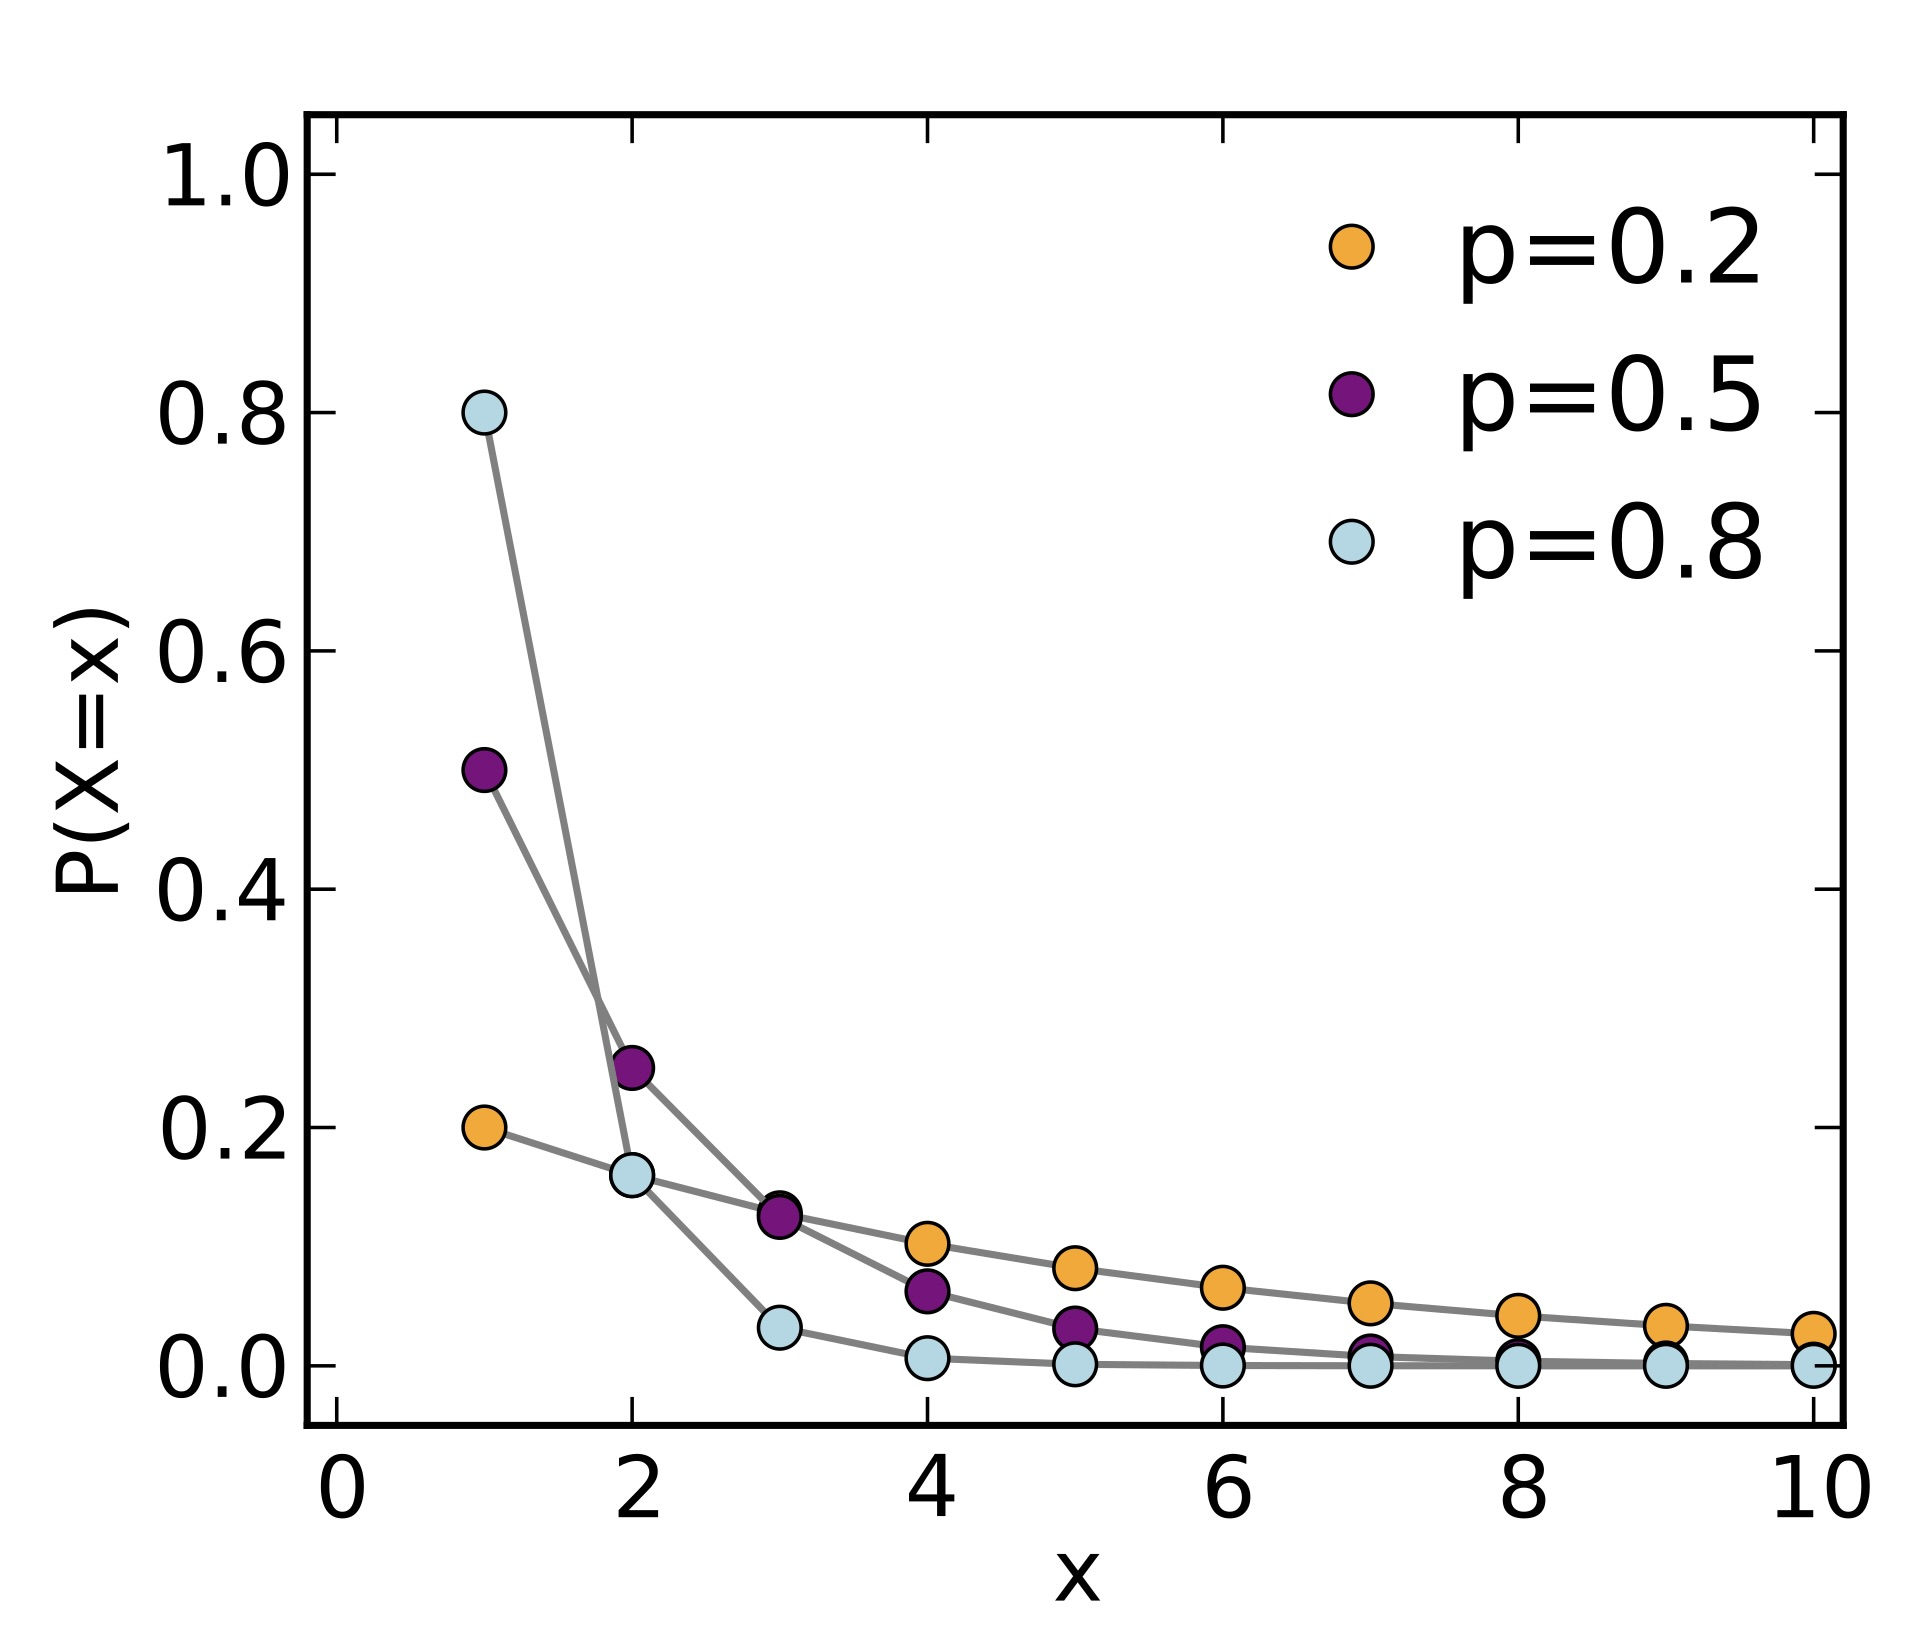
\includegraphics[width=0.65\textwidth]{assets/figures/3.jpeg}

{\small Geometric PMF: probability at integer times}
\end{center}

\column{0.53\textwidth}
\begin{center}
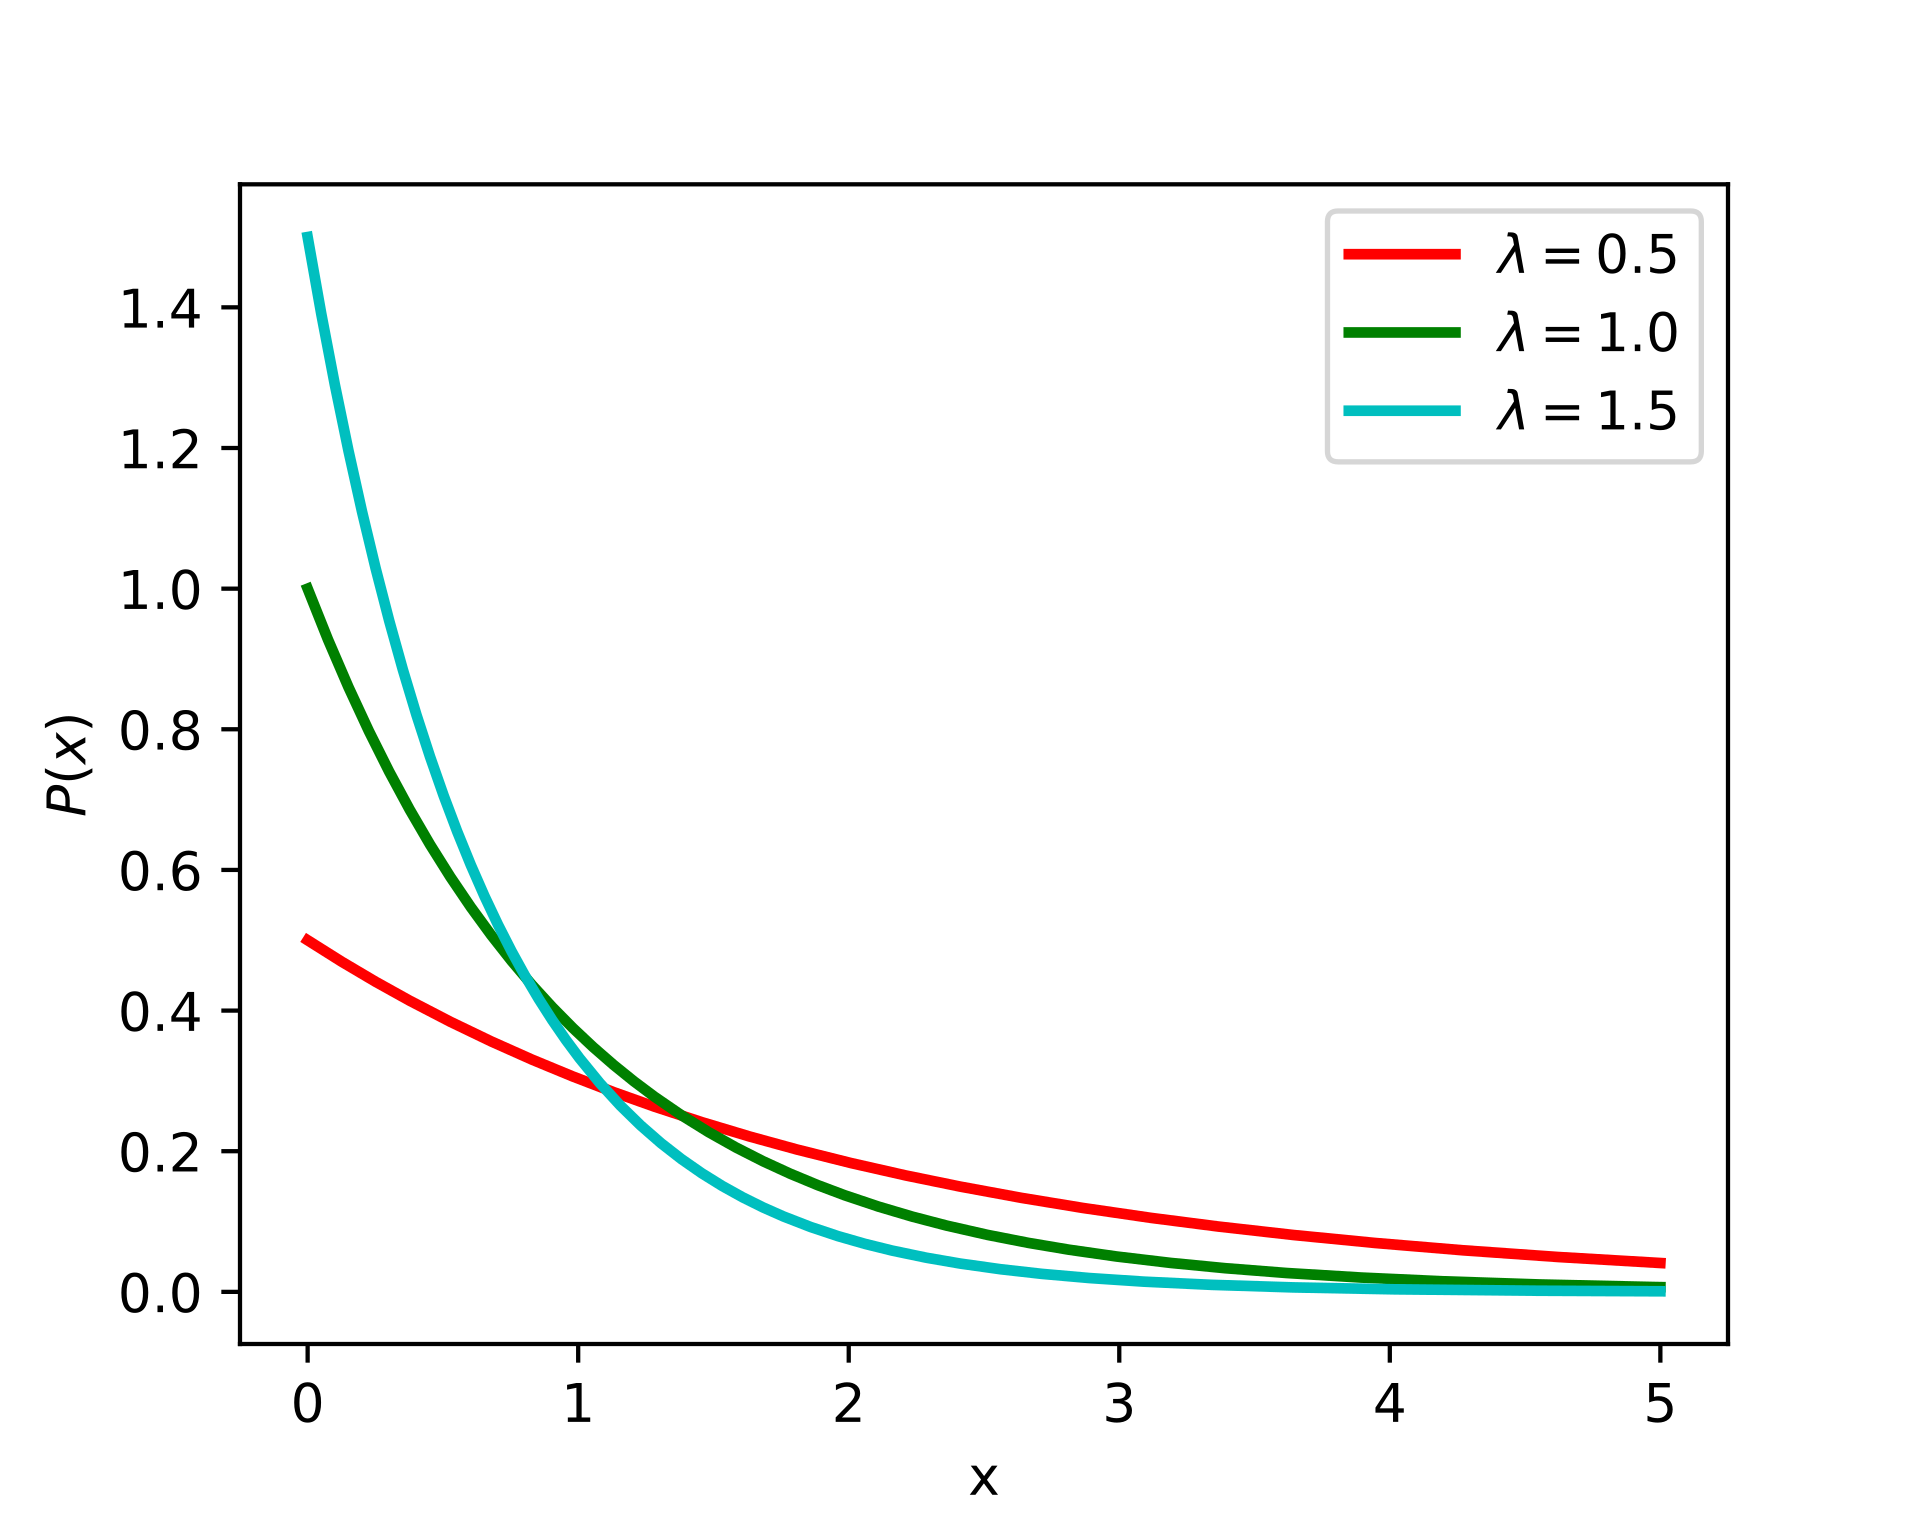
\includegraphics[width=0.65\textwidth]{assets/figures/exp-pdf.png}

{\small Exponential PDF: density over continuous time}
\end{center}
\end{columns}

\begin{center}
{\small
Geometric is the discrete-time analogue of Exponential.
}
\end{center}

\end{frame}

\begin{frame}{Summary}
\begin{itemize}
    \item The Normal distribution is bell-shaped and central in statistics.

    \item Standard Normal:
    \[
    Z\sim N(0,1).
    \]

    \item Standardization:
    \[
    \frac{X-\mu}{\sigma}\sim N(0,1).
    \]

    \item Exponential random variables model waiting times.

    \item If $X\sim \operatorname{exp}(\lambda)$, then
    \[
    \Prob(X>x)=e^{-\lambda x}.
    \]

    \item The Exponential distribution is memoryless.
\end{itemize}

\vspace{0.25cm}

\begin{keybox}{Next lecture}
Joint distributions and transformations.
\end{keybox}
\end{frame}